%%%%%%%%%%%%%%%%%%%%%%%%%%%%%%%%%%%%%%%%%
% Stylish Article
% LaTeX Template
% Version 2.1 (1/10/15)
%
% This template has been downloaded from:
% http://www.LaTeXTemplates.com
%
% Original author:
% Mathias Legrand (legrand.mathias@gmail.com) 
% With extensive modifications by:
% Vel (vel@latextemplates.com)
%
% License:
% CC BY-NC-SA 3.0 (http://creativecommons.org/licenses/by-nc-sa/3.0/)
%
%%%%%%%%%%%%%%%%%%%%%%%%%%%%%%%%%%%%%%%%%

%----------------------------------------------------------------------------------------
%	PACKAGES AND OTHER DOCUMENT CONFIGURATIONS
%----------------------------------------------------------------------------------------

\documentclass[fleqn,10pt]{SelfArx} % Document font size and equations flushed left

\usepackage[english]{babel} % Specify a different language here - english by default

\usepackage{lipsum} % Required to insert dummy text. To be removed otherwise
\usepackage[normalem]{ ulem }
\usepackage{soul}

%----------------------------------------------------------------------------------------
%	COLUMNS
%----------------------------------------------------------------------------------------

\setlength{\columnsep}{0.55cm} % Distance between the two columns of text
\setlength{\fboxrule}{0.75pt} % Width of the border around the abstract

%----------------------------------------------------------------------------------------
%	COLORS
%----------------------------------------------------------------------------------------

\definecolor{color1}{RGB}{0,0,90} % Color of the article title and sections
\definecolor{color2}{RGB}{0,20,20} % Color of the boxes behind the abstract and headings

%----------------------------------------------------------------------------------------
%	HYPERLINKS
%----------------------------------------------------------------------------------------

\usepackage{hyperref} % Required for hyperlinks
\hypersetup{hidelinks,colorlinks,breaklinks=true,urlcolor=color2,citecolor=color1,linkcolor=color1,bookmarksopen=false,pdftitle={Title},pdfauthor={Author}}

%----------------------------------------------------------------------------------------
%	ARTICLE INFORMATION
%----------------------------------------------------------------------------------------

\JournalInfo{Coupe de France de Robotique  Sujet A } % Journal information
\Archive{Nbre optimal : 4+ personnes} % Additional notes (e.g. copyright, DOI, review/research article)

\PaperTitle{CDFR 1A : Sujet d'électronique/Informatique} % Article title

\Authors{Pierre Filiol} % Authors


\Keywords{Arduino\&Raspberry --- Python\&C ---Hardware } % Keywords - if you don't want any simply remove all the text between the curly brackets
\newcommand{\keywordname}{Keywords} % Defines the keywords heading name

%----------------------------------------------------------------------------------------
%	ABSTRACT
%----------------------------------------------------------------------------------------

\Abstract{Dans le cadre du projet Coupe de France de robotique, il serait souhaitable de pouvoir visualiser les paramètres de santé du robot afin de procéder à un arrêt d'urgence si nécessaire. L'intégration de l'environnement ROS dans le robot devrait nécessiter beaucoup de ressources à la carte "intelligence" ce qui devrait se traduire par une consommation accrue et des risques d'élévation de température importants. Le système conçu devra être capable de mesurer en temps réel des informations comme le pourcentage de batterie restant et la température à plusieurs points sensibles dans l'unité centrale( fonction de veille préventive). Il est également demandé d'inclure un contrôle de 2-3 ventilateurs (type PC) afin de refroidir le robot et d'un réseau d'éclairage (type guirlande de led) pour apporter le pimp au projet. Tous les paramètres cités ci-dessus devront être envoyés vers une raspberry pi pour traitement via un protocole de communication i2C. Le dernier aspect du sujet est de crée un interface graphique en langage Python qui tournera sur la carte "intelligence" et affichera toutes les informations de santé sur un écran. }

%----------------------------------------------------------------------------------------

\begin{document}

\flushbottom % Makes all text pages the same height

\maketitle % Print the title and abstract box

\tableofcontents % Print the contents section

\thispagestyle{empty} % Removes page numbering from the first page

%----------------------------------------------------------------------------------------
%	ARTICLE CONTENTS
%----------------------------------------------------------------------------------------

\section*{Introduction} % The \section*{} command stops section numbering

\addcontentsline{toc}{section}{Introduction} % Adds this section to the table of contents

L'objectif du Sujet est, en plus de donner un gros coup de main au projet Coupe de France, de manipuler les outils qui serviront tout au long de la première année à l'Ensta-Bretagne. Les attendus du sujet permettront de se familiariser avec le langage python (UV\_1.1 UV\_1.7 UV\_2.1 UV\_2.4 UV\_2.7), l'environnement Arduino/pseudo-C (UV\_2.5) et l'électronique de base (U\_V1.7) permettant ainsi de \st{ ne pas venir en amphi} gagner du temps dans l'année ! Le travail réalisé s'inscrit directement dans les règles officielles de la Coupe de France et répondra à des problématiques comme les prévisions de points et le respect du temps en plus de s'adresser aux thématiques de conso d'énergie et d'élévation thermique.

%------------------------------------------------

\section{Proposition d'architecture}

\begin{figure*}[ht]\centering % Using \begin{figure*} makes the figure take up the entire width of the page
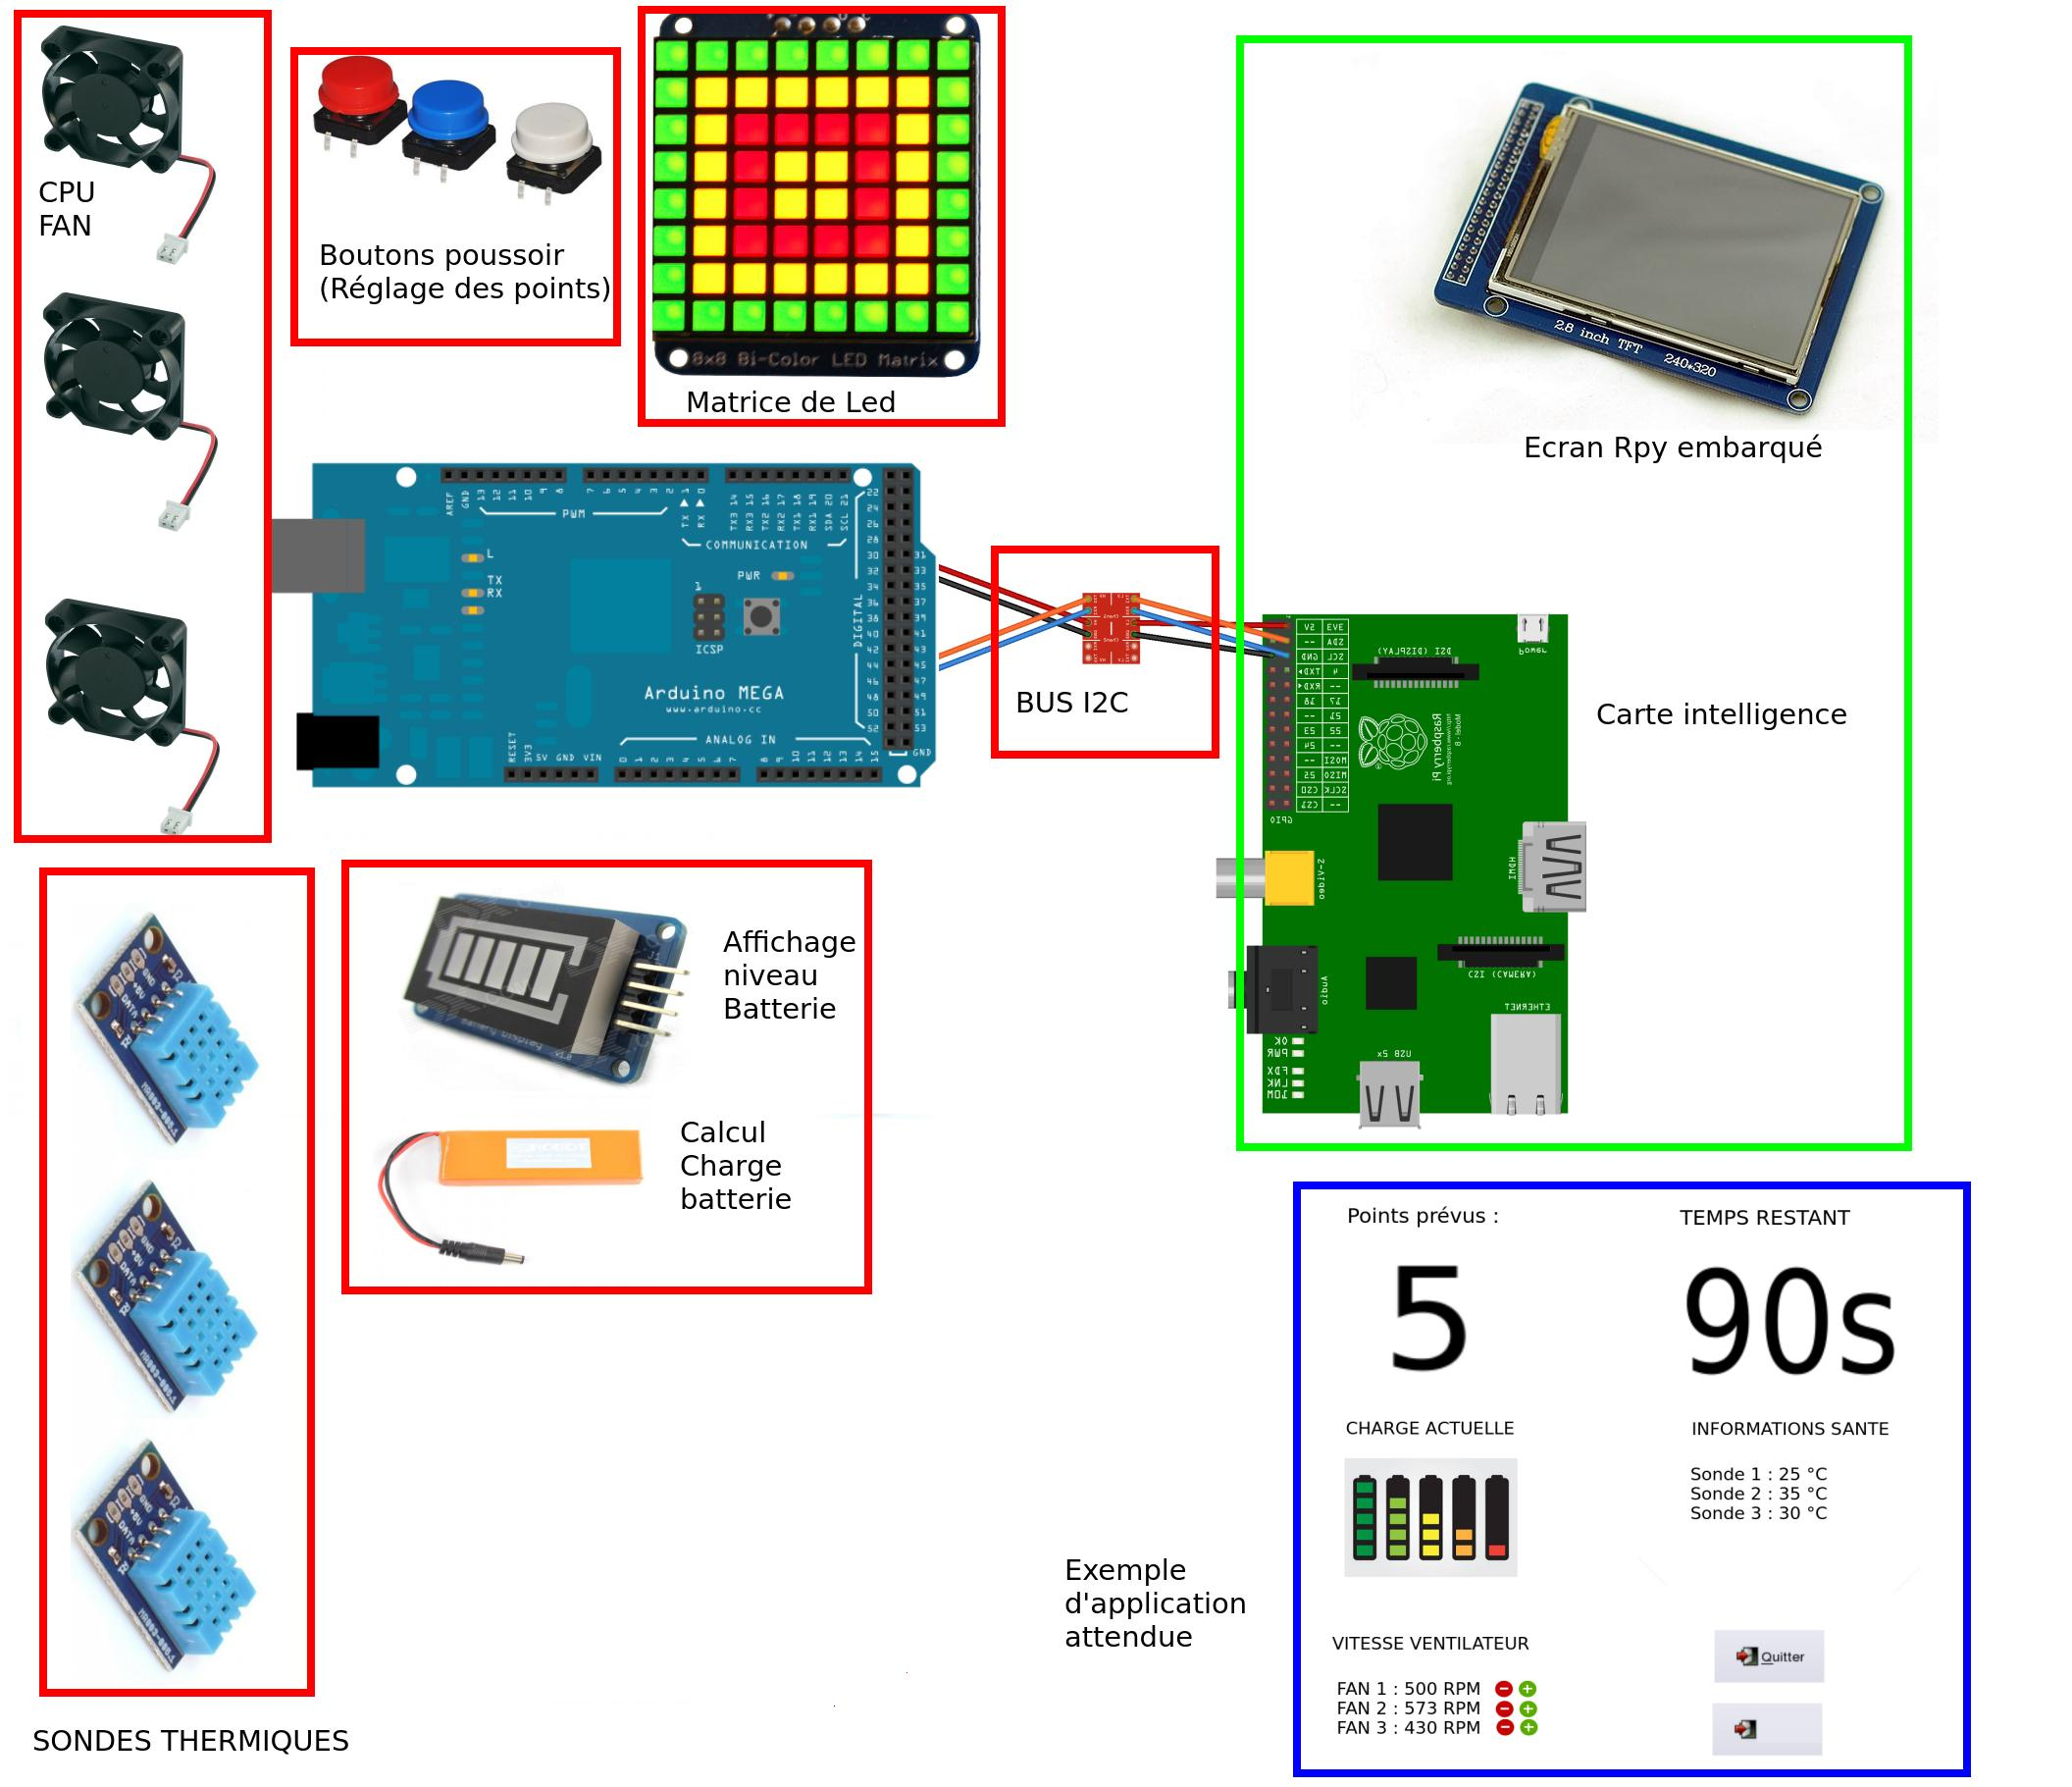
\includegraphics[width=\linewidth]{view}
\caption{Architecture proposée}
\label{fig:view}
\end{figure*}
La carte centrale sera a priori une Arduino (modèle précis à choisir en fonction des Pins requis pour implémenter toutes les fonctionnalités techniques) Le choix pourrait s'articuler entre la MEGA et la UNO. La carte devra interfacer tous les capteurs impliqués dans l'expression des fonctions techniques du tableau ci-dessous ainsi que les ventilos, cube de led etc... 

 Les fonctions de communication avec la Raspberry PI ne doivent pas être oubliées (à inclure dans le calcul des pins nécessaires lors du choix de la carte). Pour faciliter l'intégration au robot on se penchera vers le protocole de communication I2C. De nombreuses ressources existent en ligne pour programmer ce genre d'interaction sur Arduino. 
 
 
L'autre point important du sujet et de réaliser un interface graphique en Python destiné à tourner sur la carte intelligence pour visualiser les données récupérées via I2C (températures des sondes, vitesse des ventilos,points\_prévisionnels,temps restant).La bibliothèque graphique pourra être soit PyQT(utilisé à l'Ensta) ou pygame(C'est le must \^\^). Un aperçu du type d'application souhaité est disponible en fin de fichier. Bien sur tout cela constitue une base, en dehors des points obligatoires vous serez libres d'ajouter d'autres fonctionnalités si cela vous fait rire (voir quelques idées plus bas).
\\ \\ La figure ci dessous récapitule la proposition d'architecture pour le projet(soumis à changement) : 




\begin{enumerate}[noitemsep] % [noitemsep] removes whitespace between the items for a compact look
\item Carte Arduino pour l'électronique
\item Protocole I2C pour communication
\item Interface graphique d'affichage
\end{enumerate}

\section{Attendus du sujet}
\subsection{Attentes Principales}

\paragraph{Réglage du score visé}
FP1 : On pourra régler le total de point prévisionnel grâce à 3 boutons poussoirs (+1,-1,RAZ). Celui-ci sera stocké dans le code sous forme de variable prêt a être envoyé. on pourra utiliser un petit écran à cristaux pour visualiser ce paramètre depuis le chassis (plus pratique).
\paragraph{Mesures de température}
FP2 : On pourra récupérer les données thermiques à 3 endroits dans le robot. Le choix du capteur ainsi que la fréquence des relevés est laissée libre aux participants (il y a des tonnes de tutos pour ça sur internet).Ces données seront envoyées via I2C avec information sur la sonde concernée.
\paragraph{Communication I2C}
FP3 : L'Arduino devra échanger des informations avec la Raspberry pi.Voir en bas de page.
\paragraph{Contrôle de Ventilateurs}
FP4 : La carte devra controler 3 ventilateurs pour la refrigération du robot. On utilisera des FANS 5V type PC. Pour cette partie il faudra faire une petite plaque de connectique propre pour faire la liaison ventilo / pins. On souhaite pouvoir agir sur les vitesses de rotation (nécessité de réaliser une PWM).
\paragraph{Charge de la batterie}
FP5 : On affichera sur la coque (LED ou visualisateur dans l'esprit de la figure du dessus) la charge approximative de la batterie (pas besoin d'être précis au \% près. ). On utilisera le fait que la batterie se décharge a peu près linéairement et l'on peut avoir l'info sur sa charge en mesurant la tension au borne (avec AnalogRead par exemple).Plus d'info en bas de page.
\paragraph{Application de visualisation}
FP6 : Il faudra fournir une application python (Bibliothèques graphique PyGame ou PyQT) affichant toutes les informations reçues par la raspberry pi. Le rendu sera dans le style de la figure 2 (qui se veut purement fonctionnel, libre a vous de faire un style plus travaillé\^\^).
\begin{figure*}[ht]\centering % Using \begin{figure*} makes the figure take up the entire width of the page
	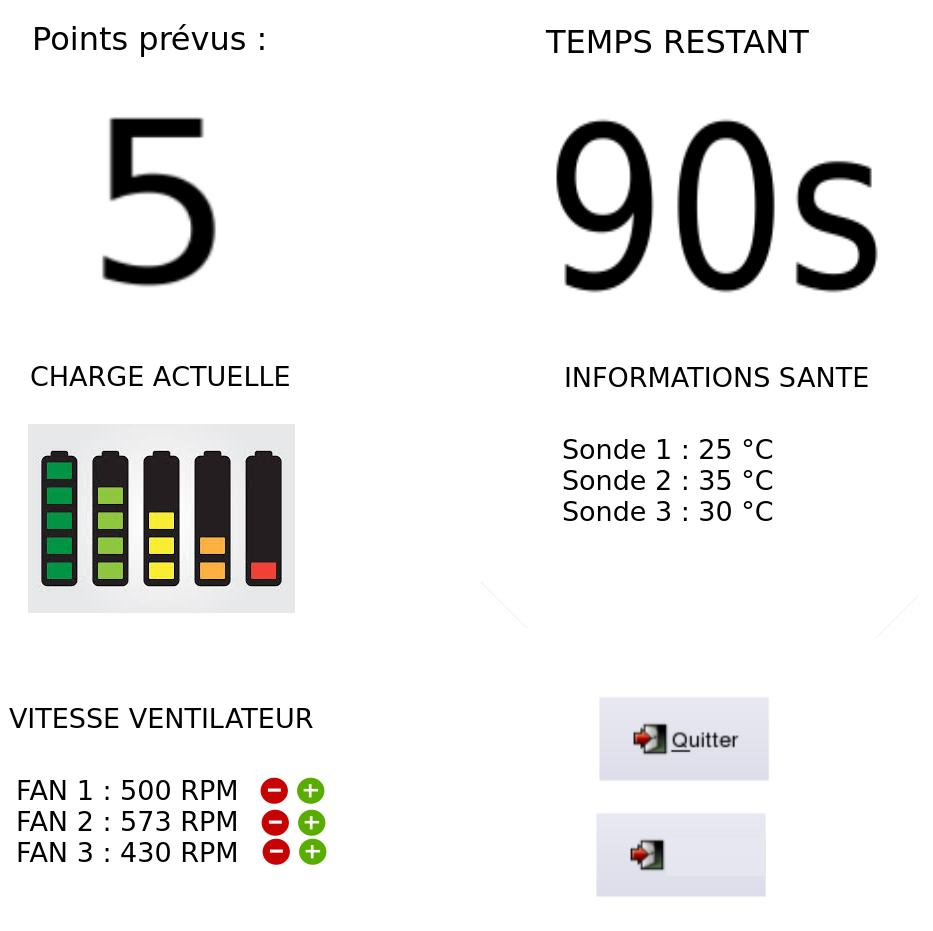
\includegraphics[width=\linewidth]{app}
	\caption{Exemple d'application}
	\label{fig:view}
\end{figure*}


\subsection{Attentes Secondaires / Pour vous amuser}
Projets completement optionnels soumis aux pins restants et aux envies
\paragraph{Pour le PIMP !}
FA1 : On réalisera un circuit d'éclairage pour le robot (du type guirlande de led). Si le budget le permet on fera ça avec des leds multicolores.De nombreux tutos sont disponibles sur le web pour ça.
\paragraph{Presque Humain(1/2)}
FA2 : Réaliser des expressions faciales pour le robot avec une matrice de LED. voir en bas.
\paragraph{Presque Humain(2/2)}
FA3 : Lire des fichiers .mp3 ou .waw avec l'arduino et donner une voix au robot.
\paragraph{Timekeeper(1/2)}
FA4 : Au top départ d'une manche (signal Raspberry envoyé via I2C ?) L'arduino commence a faire le compte à rebours de 90s et émet des bips très bruyants à la fin du temps.
\paragraph{Timekeeper(2/2)}
FA5 : Afficher ce même décompte de 90s sur l'application (façon horloge digitale)
\paragraph{Pour les sponsors ! ET LE PIIIMP}
FA6 : Faire défiler les noms/logos des sponsors dur une matrice de LED pendant les manches

%------------------------------------------------

\section{Aides et Directions}

DISCLAIMER : j'ai les pdfs pour tous les bouquins que j'indique donc si vous ne pouvez pas les trouver vous même (ce dont je doute fortement) je les ai à dispo.
\subsection{Python}

Langage de programmation pour l'application et l'I2C coté raspberry :
\begin{enumerate}[noitemsep] % [noitemsep] removes whitespace between the items for a compact look
	\item Tutoriel du site du zero sur le python (parfait pour commencer)
	\item Learning Python 5th edition publié par O'reilly (super exhaustif mais un peu indigeste)
	\item Game Programming-the L line way to learning (super tuto pour apprendre pygam et faire des jeux avec)
\end{enumerate}

\subsection{Arduino/Raspberry}

Ces plateformes sont en général très bien documentées, il est aisé de trouver de l'aide :
\begin{enumerate}[noitemsep] % [noitemsep] removes whitespace between the items for a compact look
	\item Tutoriels d'Adafruit ou autre ressources web (environnements très documentés, il est facile d'avoir des exemples)
	\item Arduino Cookbook par O'reilly (Très bien et beaucoup d'exemples)
	\item Raspberry PI cookbook par O'reilly (encore une fois très bien et beaucoup d'exemple)
\end{enumerate}

\subsection{Protocole I2C}
Débuter par la lecture de la page wiki pour comprendre de quoi il s'agit. Ensuite regarder sur internet parmi la pléthore de tutos disponibles pour une connection arduino et raspberry :

\begin{enumerate}[noitemsep] % [noitemsep] removes whitespace between the items for a compact look
	\item Tutoriels d'Adafruit et du site d'arduino
	\item Arduino Cookbook par O'reilly (Exemple à l'intérieur)
	\item Raspberry PI cookbook par O'reilly (Exemple à l'intérieur)
\end{enumerate}

\subsection{Electronique}
En vrac , Rechercher les mots clés suivants

\begin{enumerate}[noitemsep] % [noitemsep] removes whitespace between the items for a compact look
	\item Connecting CPU fans to Arduino (pour l'élaboration des plaques ventilos)
	\item Mesure charge de batterie (pour un protocole de mesure de tension batterie)
	\item Matrice de Led (pour les applications à base de ça)
\end{enumerate}


%------------------------------------------------
\phantomsection
\section*{Pour finir} % The \section*{} command stops section numbering

\addcontentsline{toc}{section}{Acknowledgments} % Adds this section to the table of contents

Plus que pour la performance le club existe pour s'éclater et apprendre des trucs. Ne pas hésiter à me demander si vous êtes bloqués et de toutes façon les séances sont là pour ça \^\^.

%----------------------------------------------------------------------------------------
%	REFERENCE LIST
%----------------------------------------------------------------------------------------

%----------------------------------------------------------------------------------------

\end{document}